\section{Methodology}
\label{chap:methodology}

%===============================================================
\subsection{AutoBrep Transformer Architecture}
%===============================================================

AutoBrep is a decoder-only transformer model with approximately 1 billion parameters, designed for autoregressive generation of Boundary Representations (B-Reps). The architecture consists of:

\begin{itemize}
	\item \textbf{35-layer Transformer decoder} with embedding dimension $d = 768$
	\item \textbf{Multi-head attention}: Processes query (\texttt{to\_q}), key, and value (\texttt{to\_v}) projection layers
	\item \textbf{Position-wise feedforward networks (MLP)}: Projections $768 \to 16384 \to 768$
	\item \textbf{Tokenization layers}: Meta tokens (complexity class), CAD tokens (face/edge/topology sequences), and geometry tokens
\end{itemize}

The model is trained on approximately 1 million B-Reps and achieves reported validity rates up to 50\% for complex geometries (up to 100 faces). It operates autoregressively, predicting the next token conditioned on all preceding tokens in the sequence.

%===============================================================
\subsection{LoRA Fine-tuning Configuration}
%===============================================================

Following the LoRA approach described in Chapter~\ref{chap:background}, we apply low-rank adapters to the AutoBrep transformer architecture. Rather than full fine-tuning, only adapter parameters are trainable while the 1B-parameter base model remains frozen.

\textbf{Adapter Placement and Dimensions:}

\[
\mathbf{z}_q = \mathbf{W}_q \cdot \mathbf{x} + \frac{\alpha}{r} \cdot \mathbf{x} \cdot \mathbf{B} \cdot \mathbf{A}
\]
where $\mathbf{A} \in \mathbb{R}^{r \times 768}$, $\mathbf{B} \in \mathbb{R}^{768 \times r}$.

AutoBrep is a 35-layer decoder-only Transformer with embedding dimension $d = 768$. We explored two adapter placement strategies:

\begin{enumerate}
	\item \textbf{Attention-Only} (Primary): Adapters inserted into query (\texttt{to\_q}) and value (\texttt{to\_v}) projection layers:

	\item \textbf{Attention + Feedforward} (Ablation): Additional adapters on the feedforward projection layers $\text{ff}: \mathbb{R}^{768} \to \mathbb{R}^{16384}$ to capture more model capacity.
\end{enumerate}


Each adapter pair at rank $r$ contributes trainable parameters. We explored two configurations:

\textbf{Attention-Only Configuration:} Across 35 layers with 2 adapters per layer ($35 \times 2 = 70$ total), with $d=768$. 

\textbf{Attention + Feedforward Configuration:} Additionally inserting adapters into the feedforward projections ($768 \to 16384 \to 768$) adds substantial capacity.

Across 35 layers: $\text{Extra} = 35 \times 17,152 \times r = 600,320 \times r$ parameters.

\begin{table}[h!]
	\centering
	\caption{LoRA Parameter Efficiency: Attention-Only vs. Attention + Feedforward}
	\label{tab:lora_params}
	\small
	\begin{tabularx}{\textwidth}{l >{\centering\arraybackslash}X >{\centering\arraybackslash}X >{\centering\arraybackslash}X}
		\toprule
		\textbf{Config} & \textbf{Rank ($r$)} & \textbf{Params (M)} & \textbf{\% Base} \\
		\midrule
		\multirow{4}{*}{\textbf{Attention}} & 4 & 0.43 & 0.043\% \\
		& 8 & 0.86 & 0.086\% \\
		& 16 & 1.72 & 0.172\% \\
		& 32 & 3.44 & 0.344\% \\
		\midrule
		\multirow{2}{*}{\textbf{Attention + FF}} & 16 & 12.12 & 1.212\% \\
		& 32 & 24.24 & 2.424\% \\
		\bottomrule
	\end{tabularx}
\end{table}

Even with feedforward adapters at $r=32$, total parameters remain $<2.5\%$, but at significant cost in memory and training time. Attention-only adapters achieved comparable results with minimal overhead.


%===============================================================
\subsection{Data Preparation Pipeline}
%===============================================================

A custom data processing pipeline converts raw STEP files (Fig.~\ref{fig:raw}) into a structured parquet dataset compatible with AutoBrep tokenization:

\par

\textbf{Processing steps:}
\begin{enumerate}
	\item \textbf{STEP Loading and Feature Extraction}: Parse CAD solids using Open Cascade, extracting faces, edges, and topology information
	\item \textbf{UV-Grid Sampling}: Sample UV-parameter spaces to create dense point clouds representing geometric surfaces 
	\item \textbf{Geometry Normalization}: Normalize coordinates to the $[-1, 1]^3$ range bounding box (Fig.~\ref{fig:preprocessed})
	\item \textbf{Serialization}: Convert numpy arrays to bytes for compact storage in the dataset
	\item \textbf{Parquet Export}: Write preprocessed geometries with corresponding bounding boxes, complexity metadata (face count), and split into train/validation (0.9/0.1) splits
\end{enumerate}

The resulting parquet dataset contains serialized geometry tensors (faces, edges) with corresponding bounding box annotations and topology metadata.

\begin{figure}[h!]
	\centering
	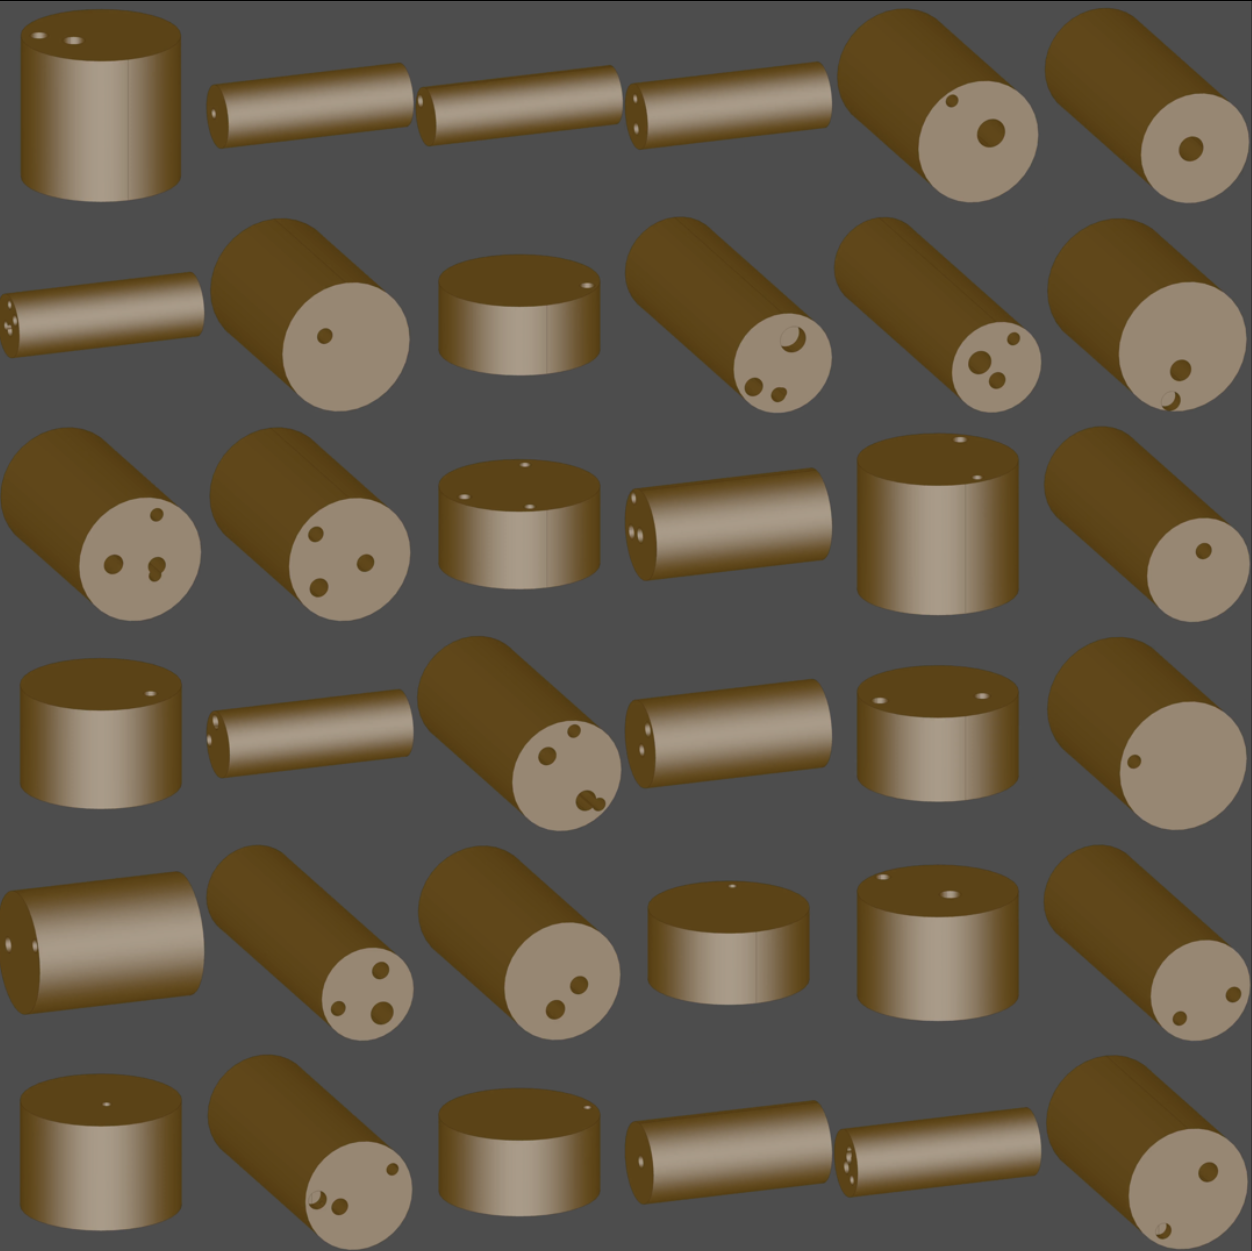
\includegraphics[width=0.5\textwidth]{figures/step_train.png}
	\caption{Raw .step file renderings of the generic cylinders with holes dataset provided by Manukai}
	\label{fig:raw}
\end{figure}

\begin{figure}[h!]
	\centering
	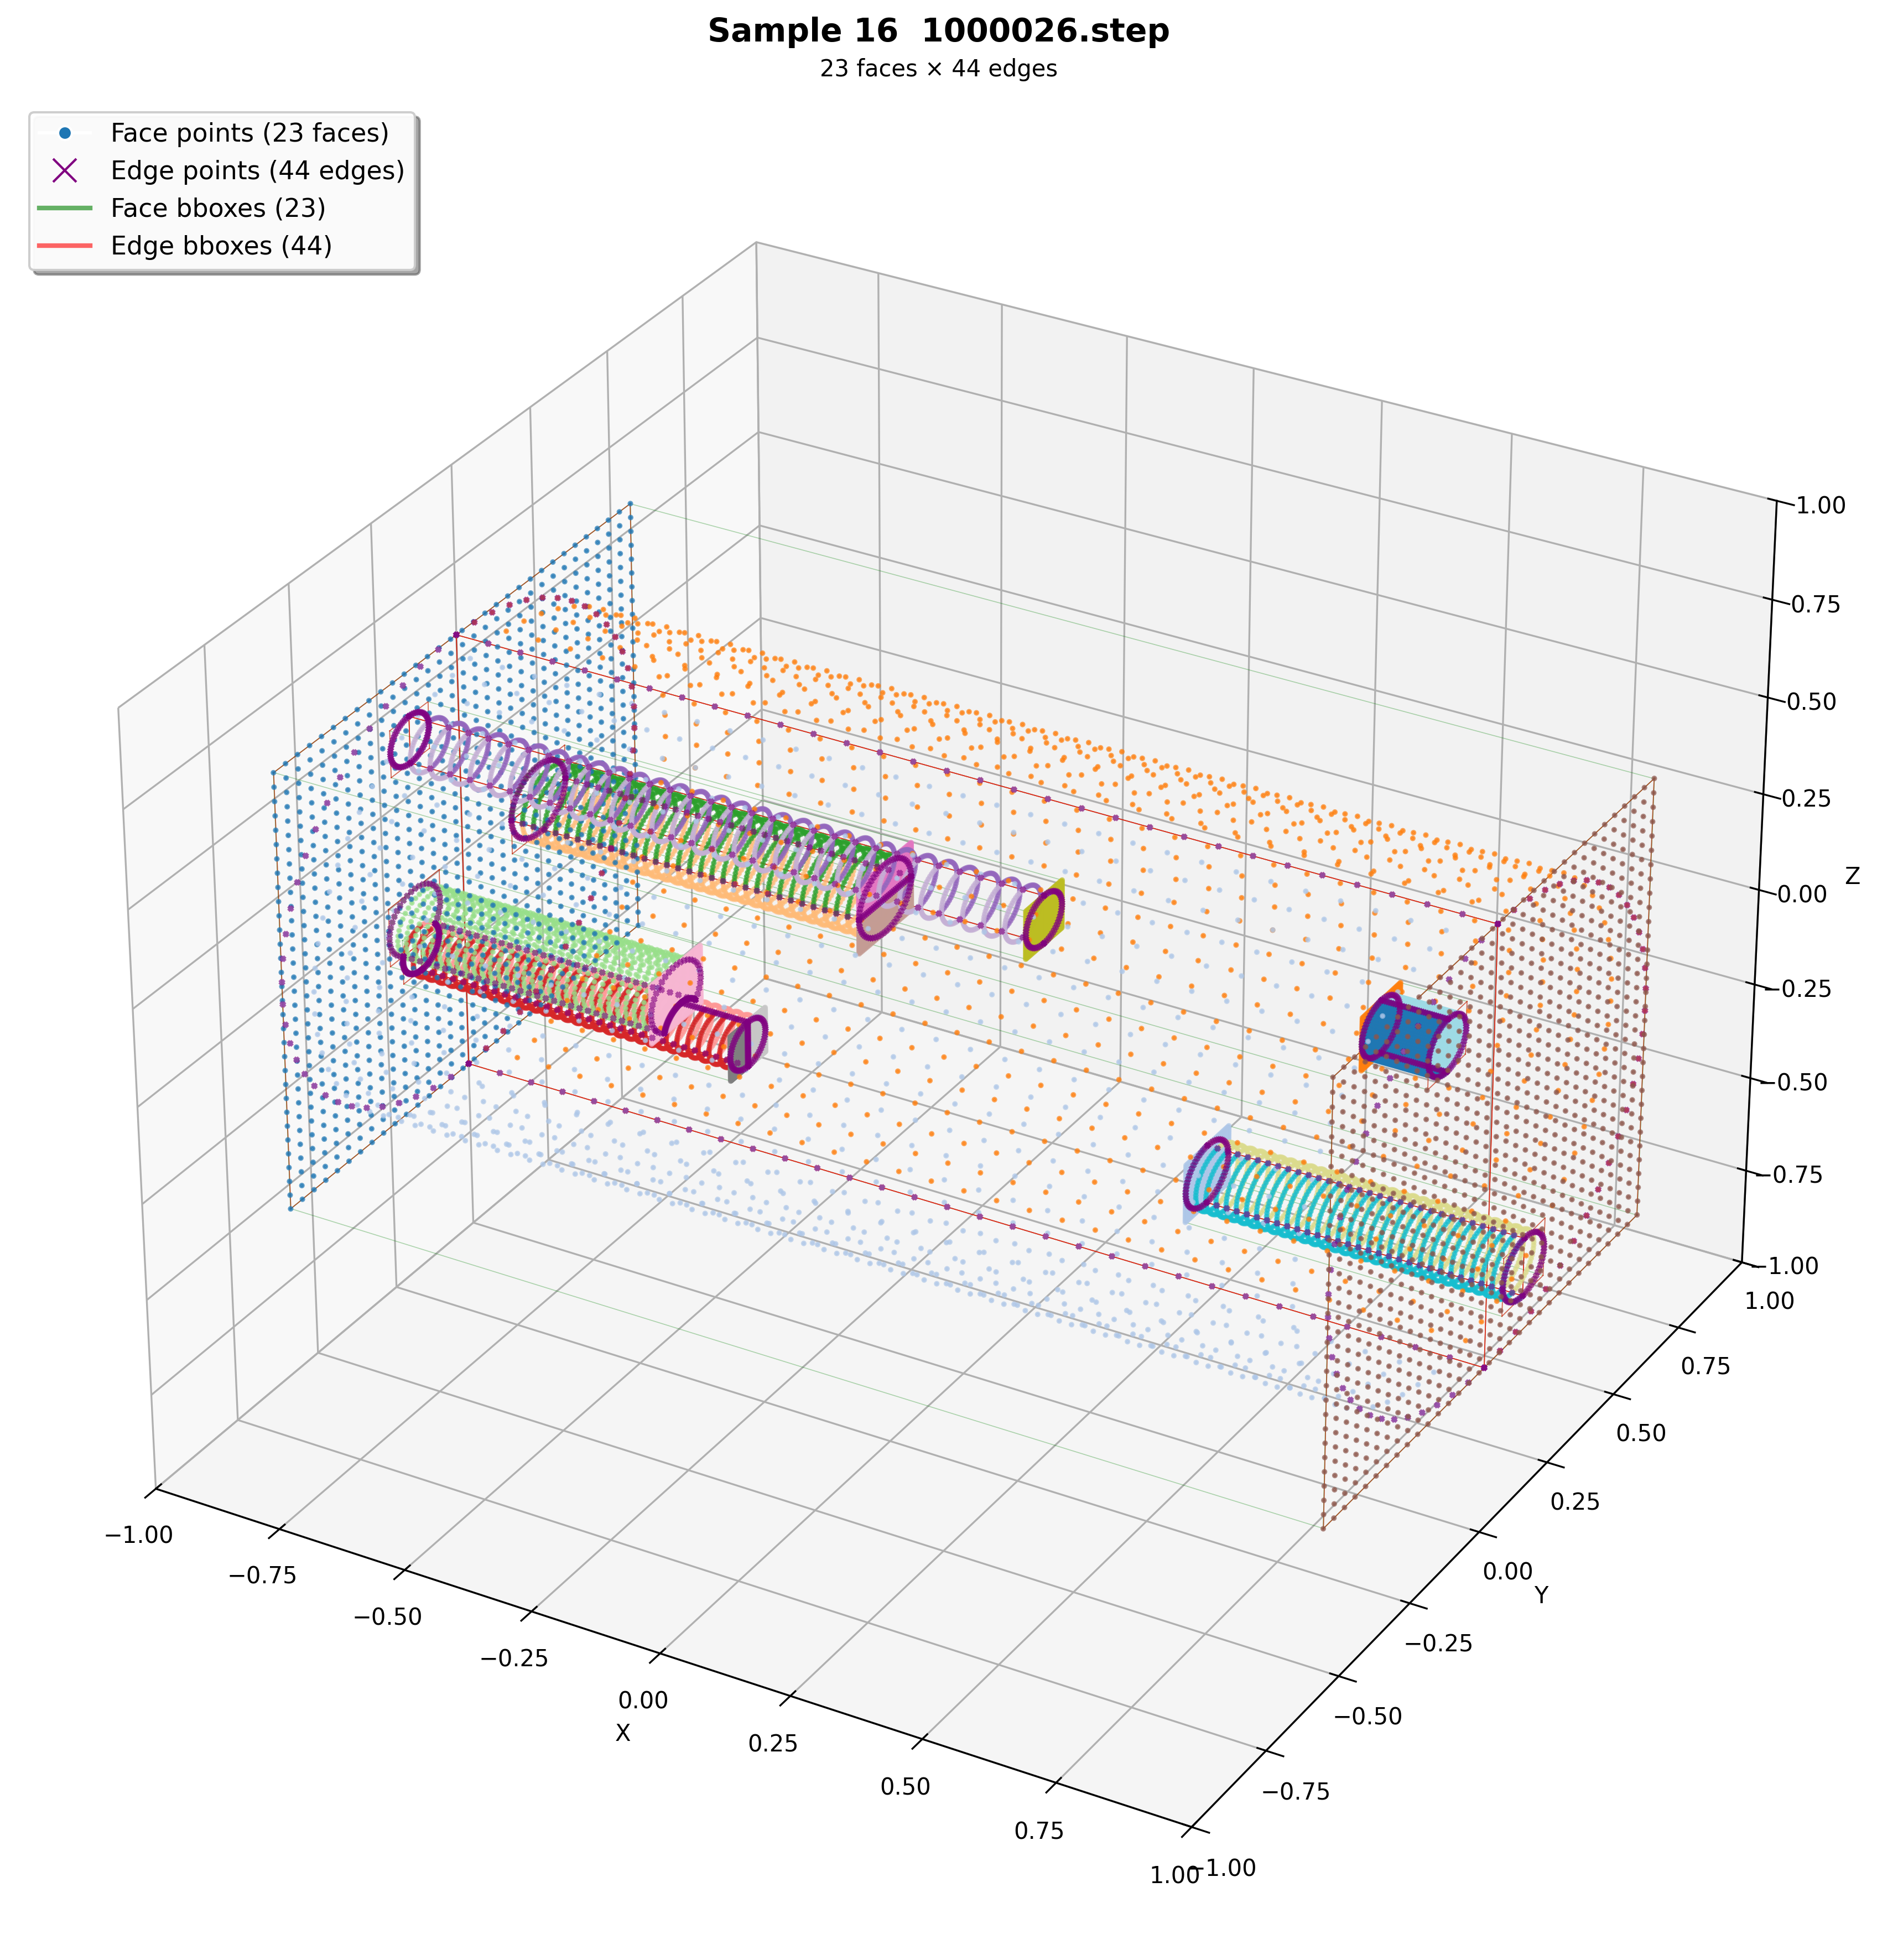
\includegraphics[width=0.5\textwidth]{figures/parquet_sample_016.png}
	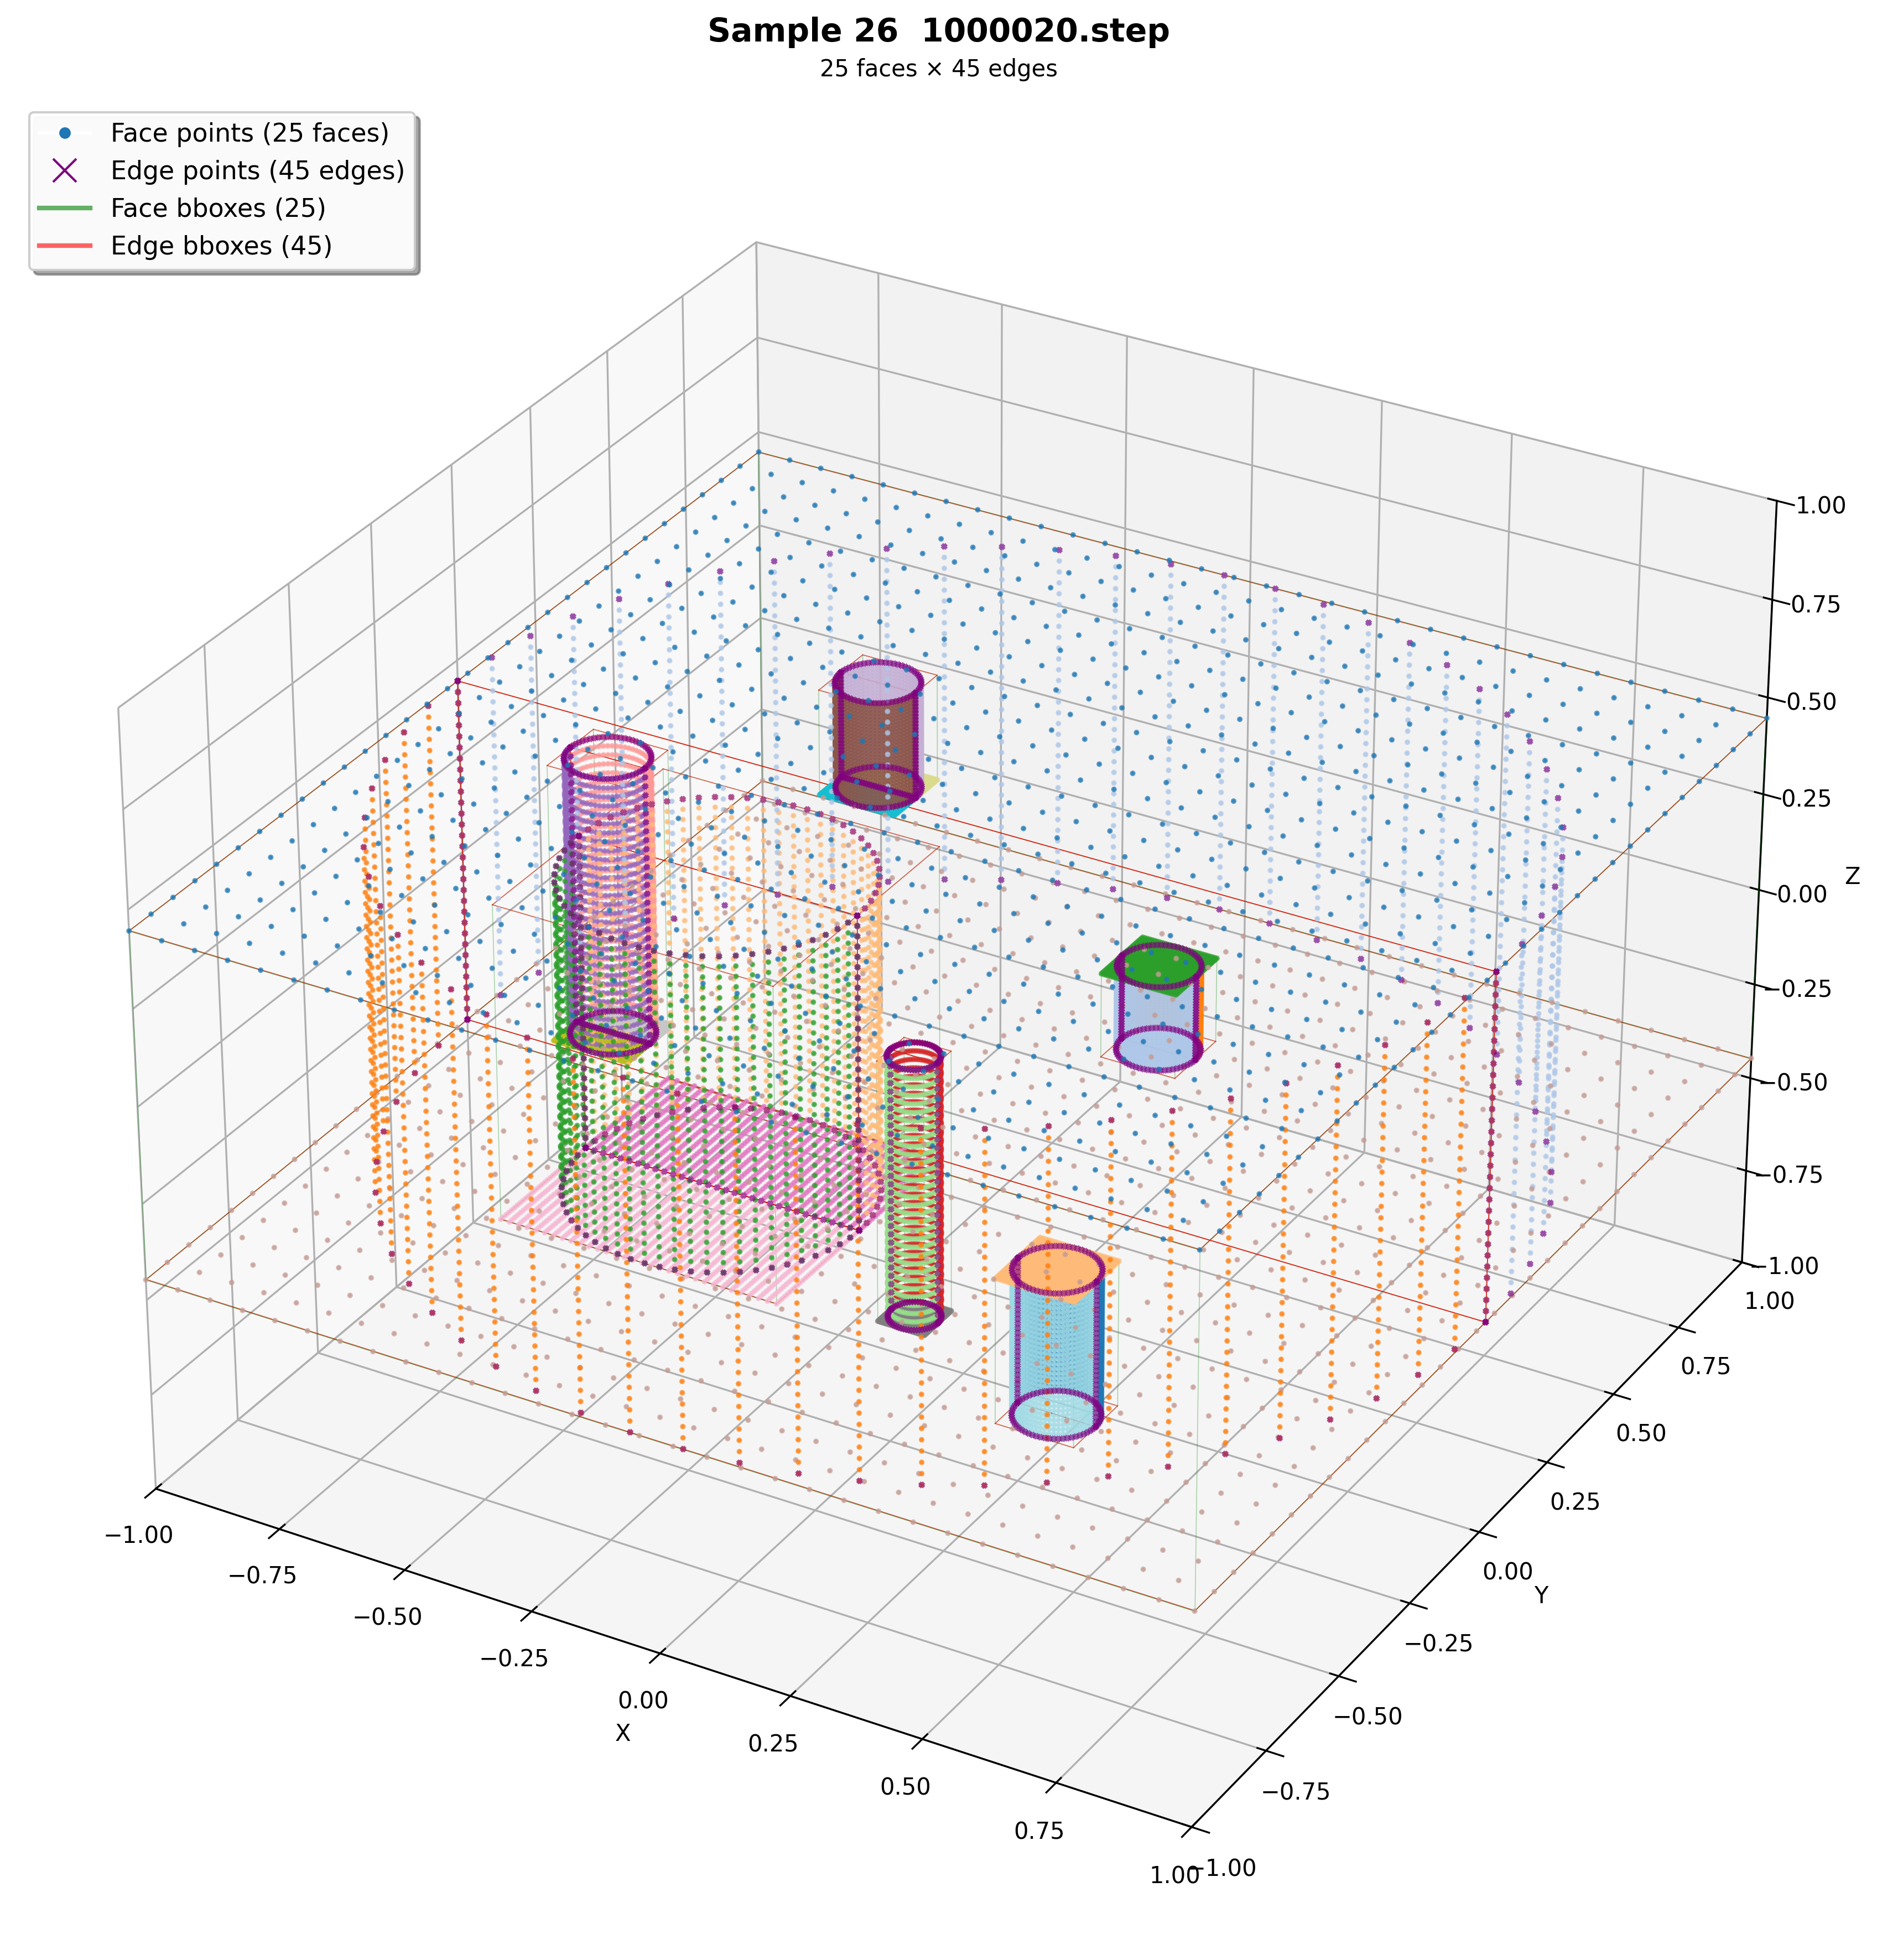
\includegraphics[width=0.49\textwidth]{figures/parquet_sample_026.png}
	\caption{Two examples of preprocessed point cloud solids of the generic cylinders with holes}
	\label{fig:preprocessed}
\end{figure}

\newpage

%===============================================================
\subsection{Training Setup}
%===============================================================

Fine-tuning is performed using the AdamW optimizer on the frozen base model with LoRA adapters as the only trainable parameters. Hyperparameter selection in table \ref{tab:training_hyperparams} follows established LoRA fine-tuning practices \cite{Hu2021lora, UnSloth2024lora}.
\par

\begin{table}[h!]
	\centering
	\caption{Training Hyperparameters following \cite{Hu2021lora}}
	\label{tab:training_hyperparams}
	\small
	\begin{tabularx}{\textwidth}{@{}l X l@{}}
		\toprule
		\textbf{Parameter} & \textbf{Value} & \textbf{Notes} \\
		\midrule
		Batch Size & 4 & Same as in Autobrep \cite{Xu2025autobrep} \\
		Number of Epochs & 4 & Typical  \\
		Learning Rate & 1e-4 to 5e-5 & Lower rates recommended for small datasets to prevent overfitting \\
		LoRA Rank & 8--32 & Balance between model capacity and parameter efficiency \\
		LoRA Alpha & $\approx 4 \times$ r & Effective scaling = $\alpha / r$; adjust for sensitivity \\
		Optimizer & AdamW & Standard choice with weight decay for regularization \\
		\bottomrule
	\end{tabularx}
\end{table}

\par

\textbf{GPU Memory Optimization:} Training on a single RTX 4090 GPU (24 GB) was enabled through three techniques: (1) casting the model to bfloat16 precision to reduce memory overhead, (2) using PyTorch's expandable memory segments
\newline (\texttt{PYTORCH\_ALLOC\_CONF=expandable\_segments:True}) to avoid fragmentation, and (3) periodic GPU cache cleanup (\texttt{torch.cuda.empty\_cache()}) every 10 batches. These techniques allowed efficient training without requiring gradient accumulation.

\par

The train and validation loss function is computed using cross-entropy loss from the AutoBrep module, which measures the divergence between predicted and ground-truth token distributions.

Training is monitored via Weights \& Biases (W\&B) for real-time loss tracking, learning rate schedules, and system metrics.

%===============================================================
\subsection{Inference and B-Rep Generation}
%===============================================================

During inference, the fine-tuned model generates B-Rep sequences autoregressively, conditioned on a complexity token. Generation is controlled via temperature sampling; top-$p$ (nucleus) sampling is kept constant at 0.95 to ensure diverse yet reasonable outputs. During training unconditional samples are created after each epoch.
Token sequences are decoded into geometric primitives (surfaces, curves) and topological relationships via the FSQ-VAE decoders. The reconstructed B-Rep geometry is then validated and assembled into watertight solids (STEP files) using the AutoBrepBuilder with the following parameters:

\begin{table}[h!]
	\centering
	\caption{Inference and B-Rep Reconstruction Parameters}
	\label{tab:reconstruction_tolerances}
	\small
	\begin{tabularx}{\textwidth}{@{}l l l@{}}
		\toprule
		\textbf{Parameter} & \textbf{Value} & \textbf{Interpretation} \\
		\midrule
		\multicolumn{3}{l}{\textit{Inference Control}} \\
		\midrule
		Complexity Token & 14--17 & 14: $<$25 faces, 15: $<$50 faces, 16: $>$50 faces, 17: random \\
		Temperature & 0.3--0.8 & Controls sampling diversity; 0.5--0.7 found optimal for fidelity+diversity \\
		\midrule
		\multicolumn{3}{l}{\textit{Reconstruction Tolerances}} \\
		\midrule
		Sewing Tolerance & $2 \times 10^{-3}$ & Max distance for edge-face sewing (watertightness) \\
		Vertex Threshold & $2 \times 10^{-3}$ & Max separation for vertex merging \\
		Z-Threshold & 0 & Z-coordinate deviation check enforced to zero (strict) \\
		\bottomrule
	\end{tabularx}
\end{table}

A B-Rep is considered valid if it passes the solid modeling kernel's validation checks: all edges are shared by exactly 2 faces (no dangling edges) and the topology forms a closed manifold (watertight) within tolerances.
